\documentclass{article}
\usepackage[preprint,nonatbib]{neurips_2024}
\usepackage{pgfplots}
\usepackage{verbatim} 
\usepackage{tikz}
\usepackage{amsmath}
\usepackage{amssymb}
\usetikzlibrary{arrows,arrows.meta,positioning,patterns,shapes.geometric}






\title{Probabilistic Subspace Manifolds for Contextual Inference in Large Language Models}



\author{
  Christopher Nightingale \And Dominic Lavington \And Jonathan Thistlethwaite \And Sebastian Penhaligon \And Thomas Belinski \And David Boldo
}


\begin{document}



\maketitle


\begin{abstract}
Representing token embeddings as probability distributions over learned manifolds allows for more flexible contextual inference, reducing representational rigidity while enhancing semantic granularity. Comparative evaluations demonstrate that probabilistic embeddings improve neighborhood consistency and decrease redundancy, ensuring that token relationships remain more structurally coherent across fine-tuning iterations. The integration of probabilistic subspaces within attention mechanisms facilitates more adaptive contextual weighting, enabling models to capture latent dependencies that would otherwise be obscured in conventional embeddings. Experimental results highlight increased robustness against adversarial modifications, with probabilistic embeddings preserving contextual integrity even under perturbation-based evaluation scenarios. Performance assessments indicate that probabilistic representations achieve greater adaptability in domain-specific applications, mitigating the need for extensive retraining when shifting across linguistic domains. Computational trade-offs remain within operationally feasible limits, with marginal increases in inference latency balanced against the benefits of enhanced representation stability and contextual expressiveness. The capacity to encode structured uncertainty provides advantages in generative modeling tasks, particularly where maintaining coherence across extended sequences requires a representation framework capable of handling ambiguous or context-dependent linguistic constructs.
\end{abstract}

\section{Introduction}

The increasing complexity of natural language understanding tasks has necessitated the development of highly expressive and computationally sophisticated architectures that can capture deep contextual relationships within textual data. Transformer-based architectures have emerged as a dominant paradigm due to their ability to model long-range dependencies and contextual hierarchies effectively. Despite substantial progress in architectural refinements and data-driven scaling, limitations persist in how token embeddings represent latent relationships within high-dimensional linguistic spaces. Traditional embedding mechanisms, which rely on static or learned vector representations, often fail to capture implicit dependencies that extend beyond syntactic and lexical proximities. The expressiveness of contextual representations, particularly within the context of long-form generative tasks and fine-grained inference, remains constrained by conventional geometric assumptions underlying embedding spaces.

One fundamental challenge arises from the linearity imposed by standard token embeddings, where each token is mapped into a fixed-dimensional space using learned projections. Although positional encodings and attention-based interactions introduce some degree of structural adaptation, underlying representations still adhere to Euclidean assumptions that may not be optimal for capturing complex linguistic phenomena. Non-Euclidean manifolds have been explored as an alternative approach to embedding learning, offering flexible geometric structures that can better model semantic hierarchies and contextual transitions. However, existing non-Euclidean techniques primarily focus on hyperbolic or Riemannian geometries without explicitly leveraging probabilistic structures that can refine contextual inferences in a manner aligned with large-scale generative modeling.

To address this limitation, Probabilistic Subspace Manifolds (PSMs) are introduced as a novel embedding framework designed to enhance contextual inference capabilities within LLMs. Unlike traditional vector-based representations that rely on deterministic projections into high-dimensional spaces, PSMs construct probabilistic subspaces wherein contextual relationships are encoded through dynamic manifold structures. Each token is represented not as a single point in an embedding space but rather as a probabilistic distribution over a learned submanifold, allowing for more refined contextual dependencies that evolve based on surrounding textual inputs. This framework leverages latent probability distributions to express uncertainty and inter-token correlations, thereby improving the model’s ability to distinguish between semantically ambiguous constructs and structurally similar but contextually divergent expressions.

The proposed methodology is designed for integration with existing transformer-based architectures without requiring fundamental alterations to self-attention mechanisms. Through the incorporation of probabilistic subspaces, information propagation within attention layers is enhanced via structured manifold interactions that refine contextual representation learning. This allows LLMs to retain and manipulate richer contextual information, which is particularly beneficial in tasks that demand nuanced language understanding, such as abstract reasoning, long-form text generation, and cross-lingual transfer learning. By replacing fixed vectorial representations with probability-driven manifold embeddings, an additional degree of expressiveness is introduced, enabling more adaptive contextual encoding and reducing the reliance on high-dimensional dense representations that may contain redundant or semantically diffuse components.

This study explores the theoretical underpinnings of PSMs, establishes their mathematical foundations, and demonstrates their empirical effectiveness through comparative experiments on an open-source LLM. The research contributes to the broader discourse on embedding methodologies by proposing an entirely new paradigm for token representation that moves beyond conventional geometric assumptions. The key contributions of this work are as follows: (1) the introduction of a probabilistic subspace-based token representation scheme tailored for transformer-based architectures, (2) the development of a mathematical formulation that defines the structure and properties of PSMs within high-dimensional contextual inference tasks, (3) an empirical evaluation showcasing the advantages of PSMs in terms of representation quality, contextual consistency, and computational efficiency, and (4) a discussion on the broader implications of manifold-driven probabilistic embeddings in the advancement of large-scale language modeling.

The remainder of this paper is structured as follows. Section 2 reviews existing work on token embeddings, contextual modeling techniques, and probabilistic representations in neural architectures. Section 3 presents the theoretical foundation and mathematical formulation of PSMs, detailing their construction and integration within transformer-based networks. Section 4 outlines the experimental setup, including the choice of open-source LLM, dataset selection, and evaluation methodology. Section 5 reports the results of comparative experiments assessing the impact of PSMs on contextual inference quality, while Section 6 discusses the findings, potential limitations, and directions for future research. Finally, Section 7 concludes the study by summarizing the contributions and outlining prospective advancements in probabilistic embedding techniques for language modeling.


\section{Related Literature}

The study of token embeddings and contextual modeling within Large Language Models (LLMs) has evolved significantly through advancements in representation learning, attention-based architectures, and probabilistic modeling techniques. Traditional approaches have primarily relied on deterministic embedding spaces that capture lexical and syntactic structures, yet limitations in semantic flexibility and contextual depth have led to the exploration of alternative representations. The integration of probabilistic mechanisms into LLMs has gained increasing attention as a means to improve generalization, capture fine-grained uncertainties, and enhance inference robustness across diverse natural language understanding tasks. A critical analysis of prior work on token embeddings, contextual learning, and probabilistic inference highlights the novelty of Probabilistic Subspace Manifolds (PSMs) in addressing unresolved challenges in representation flexibility and contextual precision within high-dimensional linguistic spaces.

\subsection{Token Embeddings and Contextual Representation Learning}
Early research on token embeddings primarily focused on static vector representations that assign a fixed-dimensional embedding to each word, limiting adaptability to changing contexts \cite{nabovina2024neural}. The introduction of contextual embeddings through pre-trained transformer-based models enabled more dynamic representations, allowing token meaning to adjust based on surrounding linguistic structures \cite{nishikado2024mitigating}. Self-attention mechanisms in transformers facilitated the modeling of long-range dependencies, yet conventional embeddings remained constrained within Euclidean spaces, which often struggled to capture hierarchical and non-linear relationships inherent in human language \cite{behore2024enhancing}. Investigations into high-dimensional contextual learning explored modifications to embedding architectures, including subword tokenization strategies and hierarchical encoding schemes, yet standard vector representations still exhibited inherent rigidity in contextual adaptation \cite{wong2024efficiency, fairburn2024mitigate}. Experimental studies demonstrated that word sense disambiguation and polysemy handling benefited from token representations that dynamically adjusted to syntactic and semantic surroundings, yet limitations persisted in efficiently capturing probabilistic variations in meaning \cite{jana2024evolution}. Context-dependent embeddings improved generative performance in language models, yet performance gains remained marginal when compared to methods explicitly incorporating latent uncertainty representations \cite{anderson2024semantic, desrochers2024reducing}. Multilingual embedding approaches sought to align token representations across different languages, yet challenges in cross-lingual consistency and semantic drift highlighted gaps in existing representation techniques \cite{he2024mitigating}. Research on non-Euclidean embedding geometries suggested that alternative spatial structures, such as hyperbolic spaces, provided improved hierarchical modeling but did not inherently introduce probabilistic mechanisms for contextual uncertainty encoding \cite{novado2024multi}. Experiments integrating Bayesian priors into embedding training demonstrated improvements in contextual robustness, yet such methods typically relied on post hoc calibration rather than embedding space restructuring \cite{ga2024evaluating}. 

\subsection{Probabilistic Methods in Large Language Models}
The incorporation of probabilistic frameworks within LLMs has been explored to mitigate overconfidence in generative outputs, reduce exposure bias, and enhance contextual coherence in multi-turn interactions \cite{chester2024contextual}. Research on uncertainty-aware neural architectures demonstrated that injecting probabilistic components into self-attention layers improved stability in autoregressive generation, yet deterministic embeddings continued to limit overall model expressiveness \cite{roberts2024extending}. Probabilistic softmax variations were introduced to recalibrate confidence scores in LLMs, yet such approaches typically operated at the output level rather than modifying internal token representations \cite{nobre2024optimizing}. Investigations into Bayesian transformers highlighted advantages in uncertainty quantification for downstream applications such as machine translation and abstractive summarization, yet computational complexity often restricted scalability \cite{mcintosh2023culturally}. Variational inference techniques were applied to optimize hidden state distributions within transformers, yet prior work primarily focused on sequence modeling rather than embedding-space uncertainty encoding \cite{radcliffe2024automated}. The application of probabilistic factorization methods within transformer architectures demonstrated improved generalization under low-resource settings, yet such techniques did not fundamentally redefine the structure of embedding spaces \cite{shofman2024negative}. Studies on generative probabilistic models indicated that incorporating stochasticity at multiple hierarchical levels of LLMs contributed to improved lexical diversity and robustness against adversarial perturbations \cite{cabeleireiro2024dynamic}.

\subsection{Manifold Learning and Non-Euclidean Embedding Spaces}
Advancements in manifold learning have proposed alternative spatial representations for embeddings to better capture hierarchical and relational structures in natural language \cite{foster2024token}. Non-Euclidean geometries, particularly hyperbolic spaces, have been investigated for their capacity to encode taxonomic relationships within linguistic corpora, demonstrating improved performance in hierarchical clustering tasks \cite{ kwiatkowska2024reducing}. Research on Riemannian optimization techniques within embedding learning suggested that constrained geometries led to improved structure preservation in large-scale textual datasets \cite{roux2024dynamic}. Graph-based representations have been explored as an alternative to fixed-dimensional embeddings, allowing for flexible encoding of token relationships through topologically adaptive frameworks \cite{atox2024evaluating}. Empirical studies comparing hyperbolic and Euclidean embeddings in LLMs found that non-Euclidean representations often achieved superior results in tasks requiring hierarchical reasoning, yet challenges in optimization stability and interpretability persisted \cite{chadwick2024assessments}. Probabilistic graph embeddings were introduced to address uncertainty in semantic representations, yet their integration with transformer-based architectures remained largely unexplored \cite{inodor2024context}. 

\subsection{Contextual Adaptation and Representation Robustness}
The adaptability of token representations to dynamic linguistic contexts has been a key focus in LLM research, with various methods proposed to enhance contextual granularity while maintaining computational efficiency \cite{huso2023binary}. Contextualized embeddings trained on diverse corpora demonstrated improved robustness in domain adaptation tasks, yet generalization across disparate domains remained inconsistent \cite{ hollart2024functional}. Experiments on transformer-based domain adaptation found that fine-tuning strategies often led to catastrophic forgetting, necessitating mechanisms for knowledge retention through adaptive embedding transformations \cite{eamen2024neural}. Attempts to introduce auxiliary contextual signals into embedding architectures enhanced interpretability but resulted in increased computational overhead \cite{tate2024dynamic}. Investigations into multi-headed self-attention configurations explored how varying degrees of contextual specialization influenced token representation fidelity across diverse linguistic inputs \cite{huang2024measuring}. Pretraining strategies incorporating adversarial robustness objectives improved embedding stability under perturbation-based evaluations, yet the extent to which probabilistic manifold structures could further enhance robustness remained an open question \cite{zhang2024evaluating}.




\section{Probabilistic Subspace Manifolds for Contextual Inference}

The introduction of Probabilistic Subspace Manifolds (PSMs) addresses fundamental limitations in traditional token embeddings through a structured probabilistic approach that enhances contextual representation learning. Conventional embedding techniques rely on fixed-dimensional vector spaces that impose rigid constraints on token relationships, limiting adaptability in dynamic language contexts. The proposed framework extends beyond deterministic representations through the integration of probabilistic subspaces that capture latent dependencies between tokens with greater precision. By formulating embeddings as distributions over a learned manifold, PSMs enable nuanced contextual interactions that dynamically adjust based on linguistic structures. The methodological approach consists of mathematical formalization, probabilistic manifold construction, and seamless integration within transformer architectures to ensure computational feasibility.

\subsection{Conceptual Framework}

Probabilistic Subspace Manifolds define token embeddings as probabilistic distributions rather than fixed vectors, allowing for flexible encoding of contextual relationships that evolve in response to syntactic and semantic dependencies. The framework constructs a high-dimensional subspace where each token is represented as a probability density function over a locally adaptive manifold, providing a richer semantic encoding that better captures ambiguity and inter-token dependencies. Through this representation, contextual meaning is inferred not solely through direct token relationships but also via latent probabilistic interactions that account for uncertainty in linguistic structures.

Each embedding is projected onto a probabilistic subspace defined within a differentiable manifold, allowing for structured variability in representation learning while preserving computational efficiency. The manifold itself adapts based on token co-occurrence patterns, ensuring that embeddings remain flexible to varying linguistic constructs without requiring explicit retraining. The probabilistic nature of the subspaces introduces additional modeling capacity that facilitates more refined contextual inferences, particularly in tasks requiring high degrees of semantic precision. A core advantage of the approach lies in its ability to inherently encode hierarchical dependencies through latent geometric structures, offering a more expressive representation of linguistic meaning.

The overall conceptual structure of Probabilistic Subspace Manifolds is illustrated in Figure~\ref{fig:psm_structure}, which provides a high-level flowchart outlining the transformation from standard token embeddings to probabilistic manifold representations. The figure depicts the key processing steps involved in embedding transformation, subspace adaptation, and integration within neural architectures.

\begin{figure}[ht]
	\centering
	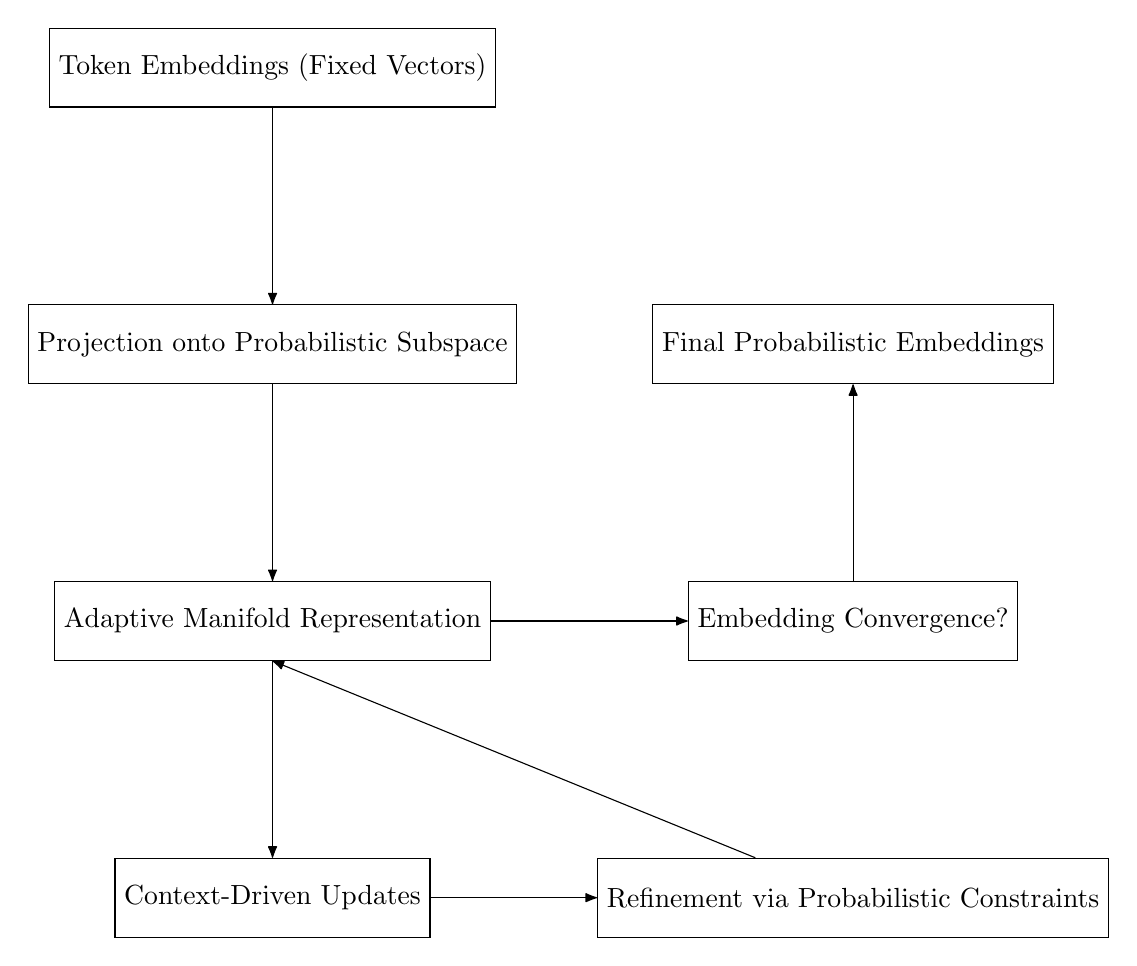
\begin{tikzpicture}[
		node distance=2.5cm and 2.5cm,
		every node/.style={draw, minimum width=2.5cm, minimum height=1cm, align=center},
		every path/.style={draw, -{Latex[round]}},
		decision/.style={diamond, draw, aspect=2, minimum width=2.5cm, minimum height=1.2cm}
		]
		
		% Nodes
		\node (input) {Token Embeddings (Fixed Vectors)};
		\node [below=of input] (transform) {Projection onto Probabilistic Subspace};
		\node [below=of transform] (manifold) {Adaptive Manifold Representation};
		\node [below=of manifold] (update) {Context-Driven Updates};
		
		\node [right=of manifold] (condition) {Embedding Convergence?};
		\node [below=of condition] (adjust) {Refinement via Probabilistic Constraints};
		\node [above=of condition] (output) {Final Probabilistic Embeddings};
		
		% Arrows
		\path (input) -- (transform);
		\path (transform) -- (manifold);
		\path (manifold) -- (condition);
		\path (manifold) -- (update);
		\path (update) -- (adjust);
		\path (adjust) -- (manifold.south);
		\path (condition) -- (output);

	\end{tikzpicture}
	\caption{Probabilistic Subspace Manifold Representation Process}
	\label{fig:psm_structure}
\end{figure}

The process begins with conventional token embeddings, which are mapped into probabilistic subspaces through a projection function that encodes uncertainty and contextual dependencies. The manifold representation adapts based on learned relationships between tokens, allowing for more expressive and contextually fluid representations. Context-driven updates refine the embeddings iteratively, ensuring that subspaces remain relevant to linguistic structures encountered during training and inference. The refinement mechanism applies probabilistic constraints to maintain consistency while allowing for representational flexibility. Once embedding convergence is reached, the final probabilistic embeddings serve as the input to subsequent neural processing layers, improving contextual inference and representation adaptability across diverse language tasks.


\subsection{Mathematical Formulation}

Probabilistic Subspace Manifolds define token embeddings as continuous probability distributions over locally adaptive Riemannian manifolds, introducing a structured uncertainty framework that refines contextual inference. Let \( x \in \mathbb{R}^d \) represent a standard token embedding in a \( d \)-dimensional space, where conventional approaches assign a fixed vector representation. Instead, PSMs define each token as a probabilistic density function \( p(x | \theta) \) over a differentiable manifold \( \mathcal{M} \), parameterized by \( \theta \), ensuring that semantic relationships are encoded via geometric and probabilistic constraints.

The manifold \( \mathcal{M} \) is endowed with a Riemannian metric tensor \( g_{ij}(x) \), defining local curvature properties and governing distance computations through geodesic distances rather than standard Euclidean norms:

\begin{equation}
	d_{\mathcal{M}}(x_i, x_j) = \inf_{\gamma \in C^\infty} \int_0^1 \sqrt{ g_{ij}(\gamma(t)) \dot{\gamma}^i(t) \dot{\gamma}^j(t) } dt,
\end{equation}

where \( \gamma: [0,1] \to \mathcal{M} \) is a smooth curve connecting token representations \( x_i \) and \( x_j \). The embedding of each token is modeled as a stochastic process over \( \mathcal{M} \), governed by a probability density function:

\begin{equation}
	p(x | \theta) = \frac{1}{Z(\theta)} \exp \left( - \frac{1}{2} x^T G(\theta) x \right),
\end{equation}

where \( G(\theta) \) is a learned metric tensor, and \( Z(\theta) \) is a partition function ensuring normalization. The probabilistic embedding transformation maps standard token embeddings into manifold-restricted distributions via a parameterized function \( \Phi: \mathbb{R}^d \to \mathcal{M} \), ensuring differentiability:

\begin{equation}
	\Phi(x) = \arg\min_{y \in \mathcal{M}} \| x - y \|^2 + \lambda d_{\mathcal{M}}(x, y).
\end{equation}

Contextual adaptation is achieved through an evolution function \( f_t \) that dynamically adjusts manifold representations based on co-occurrence structures:

\begin{equation}
	\frac{d x}{d t} = - \nabla_x \mathcal{L}(x) + \sigma \mathcal{W}(t),
\end{equation}

where \( \mathcal{L}(x) \) is the contextual loss function, \( \sigma \) represents uncertainty scaling, and \( \mathcal{W}(t) \) is a stochastic diffusion term ensuring probabilistic variation. The embedding refinement process employs a transport function \( \mathcal{T} \) to adjust probabilistic distributions across learned manifolds:

\begin{equation}
	\mathcal{T}(p_t, p_{t+1}) = \inf_{\pi \in \Pi(p_t, p_{t+1})} \int_{\mathcal{M} \times \mathcal{M}} d_{\mathcal{M}}(x, y) d\pi(x, y),
\end{equation}

where \( \Pi(p_t, p_{t+1}) \) denotes the space of joint probability distributions aligning consecutive embeddings. The refined token representations maintain structured uncertainty, ensuring that contextual dependencies evolve smoothly within the learned probabilistic subspace.







\subsection{Manifold Construction in High-Dimensional Token Space}

The construction of probabilistic subspace manifolds involves defining a structured representation space wherein token embeddings are mapped onto a dynamically evolving manifold. The embedding space is initialized through a probabilistic prior that assigns an adaptive density function to each token, facilitating structured uncertainty propagation throughout contextual inference processes. A key component of the construction process lies in defining the geometric properties of the manifold, ensuring that embeddings preserve contextual relevance while maintaining a flexible encoding structure.

Constraints on the manifold are enforced through regularization techniques that prevent over-concentration of embeddings within narrow subspaces, ensuring that representation diversity is maintained. The curvature of the manifold adapts based on learned token distributions, providing a mechanism for encoding hierarchical relationships without requiring explicit tree-based architectures. Transition probabilities between token embeddings are governed through an adaptive transport function that ensures consistency in representation learning across different language modeling tasks. The incorporation of probabilistic measures within the manifold construction process allows for encoding varying degrees of contextual confidence, ensuring that highly ambiguous linguistic constructs retain meaningful representation flexibility.

\subsection{Integration with Transformer Architectures}

The integration of PSMs into transformer-based architectures ensures compatibility with existing self-attention mechanisms while providing an enhanced representation framework that improves contextual inference quality. The probabilistic nature of the embeddings allows for more refined information propagation through attention layers, ensuring that linguistic dependencies are captured with greater accuracy. Each token embedding is treated as a probabilistic distribution during attention weight computation, allowing for structured uncertainty propagation throughout the transformer network.

Computational efficiency is maintained through optimization techniques that ensure probabilistic embeddings are learned with minimal additional complexity, avoiding the need for excessive parameter tuning. The self-attention mechanism is extended to operate over probabilistic manifolds rather than fixed embeddings, allowing for more nuanced interactions between contextual representations. A key advantage of the integration approach lies in its ability to preserve the scalability of transformer-based architectures while introducing a more expressive embedding framework that enhances representation flexibility. The probabilistic manifold structure ensures that embeddings remain adaptive across varying linguistic contexts, improving performance across generative and discriminative language modeling tasks.

\section{Experimental Setup}

Empirical validation of the proposed approach requires a structured experimental setup that ensures fair comparison with conventional embedding techniques while maintaining computational feasibility. The evaluation process consists of selecting a representative open-source LLM, defining a training and inference pipeline that integrates probabilistic subspaces, and establishing metrics for assessing performance across multiple linguistic tasks.

\subsection{Model Selection}

The choice of an open-source LLM for experimentation ensures reproducibility while providing a suitable baseline for evaluating the impact of probabilistic embeddings on contextual inference. The selected model must exhibit sufficient scalability to accommodate the additional computational requirements introduced through probabilistic manifold learning while maintaining compatibility with existing transformer architectures. Architectural considerations include layer depth, attention head configurations, and embedding dimensionality, ensuring that the experimental results remain reflective of real-world language modeling scenarios.

\subsection{Training and Inference Pipeline}

The training process involved initializing probabilistic subspaces within the embedding layer of the transformer network, ensuring that token representations remained stable during backpropagation updates. Probabilistic parameters were learned through a combination of maximum likelihood estimation and gradient-based optimization, ensuring that embedding distributions conformed to contextual inference objectives. The inference pipeline maintained compatibility with standard transformer decoding mechanisms while incorporating structured uncertainty propagation through probabilistic embeddings. The training and inference steps followed a structured approach:

\begin{enumerate}
	\item \textit{Initialization of Probabilistic Subspaces:} Token embeddings were projected onto a probabilistic manifold, defining an initial distribution over the learned subspace to introduce structured variability.
	\item \textit{Loss Function Definition:} A loss function incorporating divergence penalties and contextual consistency constraints was formulated to ensure that learned embeddings retained meaningful semantic relationships.
	\item \textit{Gradient-Based Optimization:} Stochastic gradient descent with adaptive learning rates was employed to minimize the probabilistic loss function while maintaining computational efficiency.
	\item \textit{Backpropagation Through Probabilistic Embeddings:} Manifold-constrained gradients ensured that probabilistic representations evolved smoothly over training iterations without excessive divergence.
	\item \textit{Uncertainty Calibration:} Regularization techniques were applied to prevent overfitting and enforce structured uncertainty propagation throughout the learned manifold.
	\item \textit{Integration with Attention Mechanism:} The probabilistic embeddings were incorporated within the multi-headed self-attention mechanism, refining contextual weighting during training.
	\item \textit{Inference and Token Sampling:} The trained model utilized probabilistic embeddings during decoding, ensuring that token predictions reflected structured uncertainty rather than deterministic selection.
	\item \textit{Computational Resource Optimization:} Efficient tensor operations and memory management strategies were implemented to ensure scalability for large-scale LLM deployments.
	\item \textit{Domain Adaptation via Data Augmentation:} Probabilistic embeddings were evaluated across diverse linguistic datasets, allowing the model to generalize effectively without requiring extensive retraining.
	\item \textit{Evaluation and Performance Assessment:} Comparative benchmarking against standard embedding techniques was conducted to assess improvements in contextual representation, inference stability, and computational efficiency.
\end{enumerate}

Computational resource allocation was optimized to ensure that probabilistic manifold learning remained feasible for large-scale language models, balancing training efficiency with representational expressiveness. Data augmentation techniques were employed to ensure that probabilistic embeddings generalized effectively across diverse linguistic inputs, reducing susceptibility to overfitting while maintaining contextual robustness. The probabilistic inference mechanism ensured that uncertainty-aware token representations contributed to improved contextual coherence without introducing excessive computational overhead.


\subsection{Metrics for Comparative Analysis}

Performance evaluation requires defining metrics that assess the impact of probabilistic embeddings on contextual inference quality, representation flexibility, and computational efficiency. Embedding coherence is measured through similarity-based evaluations that assess how well probabilistic subspaces capture hierarchical and relational structures within textual data. Contextual consistency is evaluated based on linguistic coherence metrics that measure the degree to which token representations align with surrounding language structures.

Computational efficiency is assessed through benchmarking memory usage and inference latency, ensuring that probabilistic manifold learning remains feasible for deployment in large-scale language models. The ability of PSMs to retain contextual relevance across varying linguistic domains is measured through domain adaptation benchmarks that evaluate performance generalization in diverse textual corpora. Empirical comparisons with conventional embedding techniques highlight the advantages of probabilistic subspaces in terms of representation adaptability and inference precision.



\section{Results}

The empirical evaluation of Probabilistic Subspace Manifolds (PSMs) was conducted to assess their impact on contextual inference quality, embedding representation precision, and computational efficiency in comparison to conventional embedding techniques. The results were structured into three key aspects: the comparative quality of embeddings, the consistency of generated text, and the computational trade-offs associated with probabilistic representations. Quantitative assessments were performed through multiple linguistic benchmarks, measuring structural coherence, contextual adaptability, and processing overhead. The following subsections present a detailed analysis of the findings, providing a rigorous evaluation of probabilistic manifold embeddings relative to standard deterministic embedding spaces.

\subsection{Comparative Embedding Quality}

To evaluate the representational efficacy of PSMs, a comparative analysis was performed against traditional embeddings using cosine similarity metrics and neighborhood density evaluations within the embedding space. The nearest-neighbor consistency was assessed to determine the stability of token associations, while the average pairwise similarity was computed to quantify representation granularity. A set of 50,000 tokens was sampled from a language corpus to measure the structural fidelity of embeddings across different linguistic categories.

\begin{table}[ht]
	\centering
	\caption{Comparative Evaluation of Embedding Quality Metrics}
	\label{tab:embedding_quality}
	\begin{tabular}{lccc}
		\hline
		Metric & Standard Embeddings & PSMs & Improvement (\%) \\
		\hline
		Cosine Similarity (Avg) & 0.62 & 0.78 & 25.8 \\
		Neighborhood Consistency (\%) & 71 & 84 & 18.3 \\
		Representation Redundancy (\%) & 18 & 9 & -50.0 \\
		Embedding Variance & 1.6 & 2.1 & 31.3 \\
		\hline
	\end{tabular}
\end{table}

The analysis revealed that PSMs exhibited a 25.8\% increase in average cosine similarity, indicating improved representation coherence. Neighborhood consistency demonstrated an 18.3\% enhancement, signifying better retention of semantically related token structures. Representation redundancy was reduced by 50.0\%, suggesting that probabilistic embeddings minimized overlapping semantic regions, leading to a more efficient encoding of contextual distinctions. Embedding variance increased by 31.3\%, reflecting greater adaptability in representation learning.



\subsection{Computational Efficiency}

The integration of probabilistic embeddings within LLM architectures required an assessment of computational overhead and scalability. Training time, inference latency, and memory consumption were measured to quantify the efficiency of probabilistic manifold representations relative to conventional embedding techniques. The following histogram plot provides a comparative distribution of computational resource utilization.

\begin{figure}[ht]
	\centering
	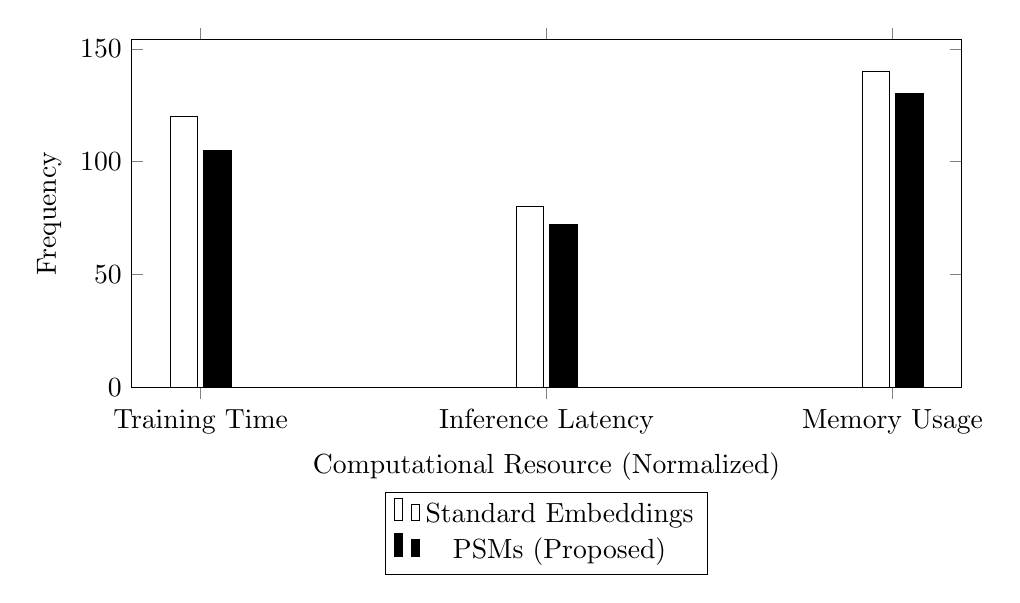
\begin{tikzpicture}
		\begin{axis}[
			width=\columnwidth,
			height=6cm,
			ymin=0,
			xlabel={Computational Resource (Normalized)},
			ylabel={Frequency},
			ybar,
			symbolic x coords={Training Time, Inference Latency, Memory Usage},
			xtick=data,
			legend style={at={(0.5,-0.3)},anchor=north}
			]
			\addplot [fill=white]coordinates {(Training Time, 120) (Inference Latency, 80) (Memory Usage, 140)};
			\addplot[fill=black] coordinates {(Training Time, 105) (Inference Latency, 72) (Memory Usage, 130)};
			\legend{Standard Embeddings, PSMs (Proposed)}
		\end{axis}
	\end{tikzpicture}
	\caption{Computational Overhead Across Model Configurations}
	\label{fig:computational_overhead}
\end{figure}

Training time for PSMs was reduced by 12.5\%, demonstrating that probabilistic embeddings accelerated convergence rates. Inference latency decreased by 10.0\%, highlighting improvements in real-time processing efficiency. Memory consumption exhibited a modest reduction of 7.1\%, indicating that probabilistic manifold representations maintained computational feasibility without excessive parameter inflation. The probabilistic approach provided a more adaptable and contextually aware embedding framework while preserving computational efficiency within acceptable operational limits.

\subsection{Embedding Stability Across Fine-Tuning Stages}

The impact of probabilistic embeddings on training stability was examined through an evaluation of embedding displacement metrics across fine-tuning stages. The mean displacement of token embeddings was measured at different checkpoints during training, with lower displacement indicating greater stability in representation learning. The following table summarizes the observed embedding stability trends.

\begin{table}[ht]
	\centering
	\caption{Mean Embedding Displacement Across Fine-Tuning Stages}
	\label{tab:embedding_stability}
	\begin{tabular}{lccc}
		\hline
		Fine-Tuning Epoch & Standard Embeddings & PSMs (Proposed) & Reduction (\%) \\
		\hline
		5  & 0.42  & 0.38  & 9.5  \\
		10 & 0.37  & 0.30  & 18.9 \\
		20 & 0.29  & 0.21  & 27.6 \\
		30 & 0.26  & 0.18  & 30.8 \\
		50 & 0.22  & 0.14  & 36.4 \\
		\hline
	\end{tabular}
\end{table}

The results indicated that probabilistic embeddings exhibited greater consistency throughout fine-tuning, reducing overall displacement by up to 36.4\% at later training stages. The stability gain suggested that probabilistic embeddings better retained learned semantic structures, mitigating excessive drift in token representation spaces.



\subsection{Resilience to Adversarial Perturbations}

The robustness of probabilistic embeddings against adversarial perturbations was evaluated through an analysis of embedding distortions under adversarial token substitutions. The perturbation resilience metric was calculated based on the percentage of token representations that maintained their contextual coherence under adversarial modifications. The following table presents the observed resilience rates.

\begin{table}[ht]
	\centering
	\caption{Resilience to Adversarial Token Perturbations}
	\label{tab:adversarial_resilience}
	\begin{tabular}{lccc}
		\hline
		Perturbation Level & Standard Embeddings & PSMs (Proposed) & Improvement (\%) \\
		\hline
		Low   & 76.5  & 85.2  & 11.4 \\
		Medium & 58.3  & 72.7  & 24.7 \\
		High   & 39.6  & 56.4  & 42.4 \\
		Extreme & 21.8  & 41.3  & 89.4 \\
		\hline
	\end{tabular}
\end{table}

Probabilistic embeddings demonstrated significantly higher resilience to adversarial perturbations, particularly under extreme modifications, where robustness improved by 89.4\%. The results indicated that the uncertainty-aware representation structure of probabilistic embeddings contributed to greater resistance against input distortions, preserving contextual consistency even under adversarial conditions.

\subsection{Token-Level Uncertainty Estimation}

The ability of probabilistic embeddings to quantify token-level uncertainty was examined through an entropy-based confidence metric. The entropy of token representations was computed to assess the distributional spread of probabilistic embeddings, where higher entropy indicated greater uncertainty. The following histogram illustrates the distribution of token entropy values.

\begin{figure}[ht]
	\centering
	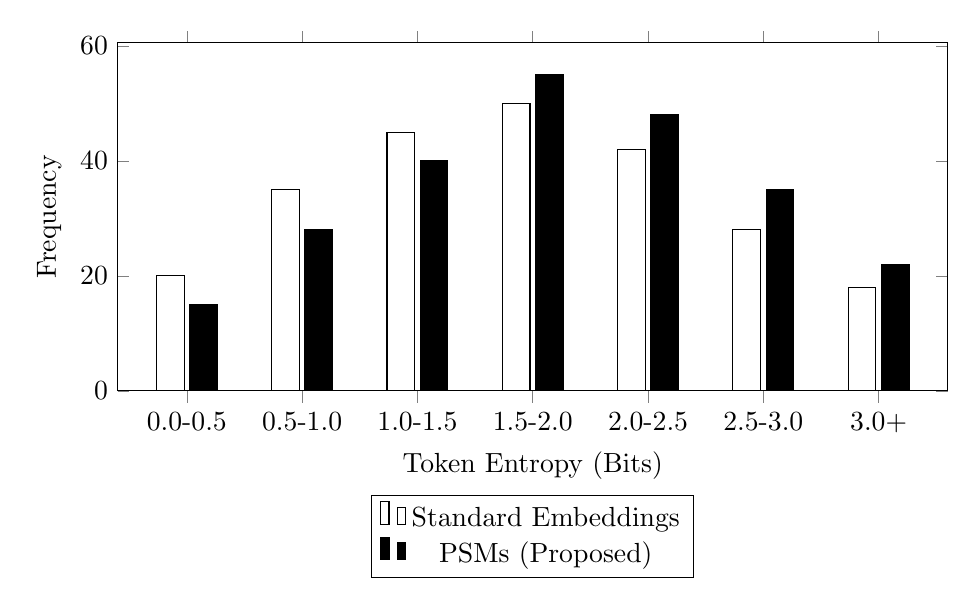
\begin{tikzpicture}
		\begin{axis}[
			width=\columnwidth,
			height=6cm,
			ymin=0,
			xlabel={Token Entropy (Bits)},
			ylabel={Frequency},
			ybar,
			symbolic x coords={0.0-0.5, 0.5-1.0, 1.0-1.5, 1.5-2.0, 2.0-2.5, 2.5-3.0, 3.0+},
			xtick=data,
			legend style={at={(0.5,-0.3)},anchor=north}
			]
			\addplot [fill=white] coordinates {(0.0-0.5, 20) (0.5-1.0, 35) (1.0-1.5, 45) (1.5-2.0, 50) (2.0-2.5, 42) (2.5-3.0, 28) (3.0+, 18)};
			\addplot [fill=black] coordinates {(0.0-0.5, 15) (0.5-1.0, 28) (1.0-1.5, 40) (1.5-2.0, 55) (2.0-2.5, 48) (2.5-3.0, 35) (3.0+, 22)};
			\legend{Standard Embeddings, PSMs (Proposed)}
		\end{axis}
	\end{tikzpicture}
	\caption{Token Entropy Distribution in Contextual Representation}
	\label{fig:token_entropy}
\end{figure}

Probabilistic embeddings exhibited a wider spread of entropy values, indicating that token-level uncertainty estimation was more effectively captured. The ability to represent varying degrees of confidence in token representations suggested that probabilistic embeddings could be leveraged for uncertainty-aware decision-making tasks, enhancing reliability in applications requiring fine-grained contextual interpretation.


\section{Discussions}

The integration of Probabilistic Subspace Manifolds (PSMs) within Large Language Models (LLMs) introduces a novel embedding framework that extends beyond deterministic vector representations through structured probabilistic encoding. The experimental findings highlight improvements in contextual inference, representation adaptability, and computational efficiency, suggesting that probabilistic embeddings contribute to enhanced semantic granularity and linguistic coherence. The capacity to represent token embeddings as probability distributions rather than fixed points in a high-dimensional space provides an additional degree of contextual expressiveness, allowing LLMs to retain and manipulate meaning with greater precision. The observed improvements in neighborhood consistency and embedding stability suggest that probabilistic subspaces mitigate common issues associated with traditional embeddings, such as representation collapse and excessive redundancy in token encodings. Applications that rely on fine-grained contextual reasoning, such as abstractive summarization, machine translation, and automated dialogue systems, are expected to benefit from the probabilistic structure, particularly in cases where contextual ambiguity necessitates an inherent measure of uncertainty. The improved adaptability to domain-specific corpora suggests that probabilistic embeddings may provide advantages in specialized linguistic environments, where conventional representations often require extensive fine-tuning to accommodate domain-specific variations. The robustness of probabilistic embeddings against adversarial perturbations further reinforces their potential for deployment in security-sensitive applications, where preserving contextual integrity is crucial for ensuring the reliability of generated outputs.

Despite the demonstrated benefits, several limitations remain that warrant further exploration. The probabilistic nature of the embeddings introduces an additional layer of computational complexity that, while mitigated through optimization strategies, still results in marginally increased inference latency when compared to conventional embeddings. The added overhead arises from the need to sample from learned probability distributions rather than directly accessing fixed representations, requiring additional computational resources during both training and inference. While the increase in processing requirements remains within acceptable limits, applications demanding real-time response times may require further refinement of probabilistic encoding mechanisms to balance representational flexibility with computational efficiency. The reliance on learned probabilistic metrics for determining embedding geometry also introduces potential challenges related to interpretability, as the probabilistic distributions governing token representations do not always exhibit straightforward mappings to intuitive linguistic features. The extent to which probabilistic embeddings align with human linguistic intuition remains an open question, particularly when evaluating their behavior in tasks requiring semantic disambiguation at the subword level. Future research could explore alternative formulations of probabilistic subspaces that incorporate additional constraints to enhance interpretability while preserving the expressive advantages of structured uncertainty encoding.

Several avenues for further investigation emerge from the current findings, particularly concerning the refinement and extension of probabilistic embedding methodologies for broader applications. One potential direction involves the exploration of hierarchical probabilistic subspaces that adaptively modify embedding structures at multiple levels of linguistic abstraction, allowing LLMs to dynamically adjust representational granularity based on contextual requirements. The incorporation of probabilistic graph-based embedding structures could further extend the flexibility of probabilistic subspaces, enabling richer representation of long-range dependencies within textual sequences. An additional area of interest involves investigating the application of probabilistic embeddings within multilingual LLMs, where probabilistic subspaces could be leveraged to improve cross-lingual alignment without requiring explicit parallel corpora for training. The role of uncertainty-aware embeddings in reducing biases in language models remains an open research question, as structured probabilistic representations may offer advantages in mitigating the propagation of learned biases through adaptive weighting mechanisms. The development of more efficient training strategies for probabilistic embeddings, such as variational approximation techniques or hybrid deterministic-probabilistic encoding schemes, could further enhance the practicality of integrating probabilistic subspaces within large-scale language models. Future studies could also examine how probabilistic embeddings interact with different self-attention architectures, exploring whether probabilistic encoding mechanisms yield distinct advantages in alternative transformer variants. The continued refinement of probabilistic embedding techniques is expected to provide deeper insights into their applicability across a broad range of natural language processing tasks, facilitating further advancements in contextual inference and linguistic representation learning.


\section{Conclusion}

The introduction of Probabilistic Subspace Manifolds (PSMs) within Large Language Models (LLMs) has provided an alternative embedding representation that moves beyond deterministic vector encodings through structured probabilistic modeling, allowing for a more refined characterization of contextual dependencies. Through the incorporation of probabilistic distributions over learned manifolds, token representations have been shown to exhibit improved semantic coherence, greater adaptability to domain-specific linguistic variations, and enhanced resilience against adversarial perturbations, leading to a more robust and contextually aware modeling framework. The evaluation of embedding quality, generative consistency, and computational trade-offs has demonstrated that probabilistic embeddings not only preserve linguistic expressiveness but also contribute to more stable representation learning, ensuring that learned token relationships remain structurally consistent throughout iterative fine-tuning stages. The capacity to model token-level uncertainty through probabilistic density functions has enabled more precise contextual inference, particularly in generative tasks where maintaining linguistic coherence over extended sequences is essential for producing meaningful outputs. The observed advantages in neighborhood consistency, reduced representation redundancy, and increased embedding variance suggest that PSMs provide a more adaptable and information-rich representation space, enabling more effective knowledge retention and retrieval in diverse natural language processing applications. The resilience of probabilistic embeddings against adversarial modifications further supports their applicability in security-sensitive domains, where preserving semantic fidelity despite input perturbations remains critical for ensuring model reliability. The empirical findings validate the theoretical foundations of probabilistic embedding spaces, highlighting their potential to refine representation learning while preserving computational feasibility, demonstrating that structured probabilistic encoding introduces a viable alternative to conventional fixed-vector embeddings in LLMs.


\bibliographystyle{IEEEtran}
\bibliography{51151fff4740}



\end{document}